\documentclass[a4paper, 10pt, final, garamond]{book}
\usepackage{cours-preambule}

\makeatletter
\renewcommand{\@chapapp}{M\'ecanique -- chapitres}
\renewcommand\thechapter{6 et 7}
\makeatother
\renewcommand{\theequation}{7.\arabic{equation}}
\renewcommand{\thefigure}{\arabic{figure}}

\hfuzz=5.002pt

% \toggletrue{student}
% \toggletrue{corrige}
% \renewcommand{\mycol}{black}
\renewcommand{\mycol}{gray}

\begin{document}
% \setcounter{chapter}{0}

\settype{enon}
\settype{solu_prof}
\settype{solu_stud}

\chapter{TD~: moment cin\'etique et forces centrales}

\section{Gravimètre de \textsc{Holweck-Lejay}}

\enonce{%
	\noindent
	\begin{minipage}[]{0.25\linewidth}
		\begin{center}
			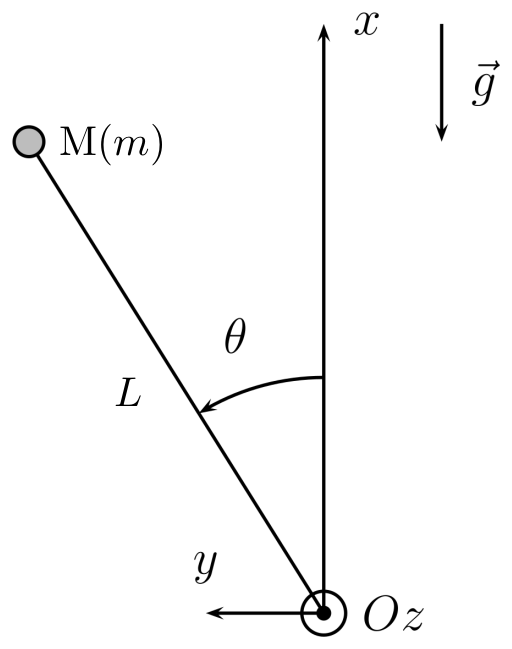
\includegraphics[width=\linewidth]{holweck-plain_m}
		\end{center}
	\end{minipage}
	\hfill
	\begin{minipage}[]{0.70\linewidth}
		Une masse ponctuelle $m$ est placée à l'extrémité M d'une tige de masse
		négligeable et de longueur $L = \OMr$, articulée en O et mobile dans un plan
		vertical. Un ressort «~spirale~» (non représenté sur la figure) exerce sur M,
		via la tige, un couple de rappel (notion abordée au chapitre 8) équivalent à
		un moment de force $\Mcf_{\Or} = -C\th\uz$, avec $C>0$.
	\end{minipage}
}

\QR{%
	Déterminer, par l'application du théorème du moment cinétique par
	rapport à l'axe $(\Or z)$, l'équation différentielle vérifiée par
	$\th$.
}{%
	\smallbreak
	\vspace{-15pt}
	\noindent
	\begin{minipage}[]{.70\linewidth}
		\begin{itemize}
			\bitem{Système}~: {masse}, repérée par M($m$).
			\bitem{Référentiel}~: terrestre supposé galiléen.
			\bitem{Repère}~: cylindrique $(\Or,\ur,\ut,\uz)$ (voir schéma).
			\bitem{Repérage}~:
			\vspace{-20pt}
			\begin{align*}
				\OM & = L \ur                \\
				\vf & = L\tp\ut              \\
				\af & = L\tpp\ur - L\tp^2\ur
			\end{align*}
			\bitem{BDF}~:
			\vspace{-10pt}
			\[
				\left\{
				\begin{array}{ll}
					\Pf & = -mg \ux = mg(-\cos(\th)\ur + \sin(\th)\ut)
					\\
					\Ff & \text{inconnue}
				\end{array}
				\right.
			\]
		\end{itemize}
	\end{minipage}
	\begin{minipage}[c]{.20\linewidth}
		~
		\begin{center}
			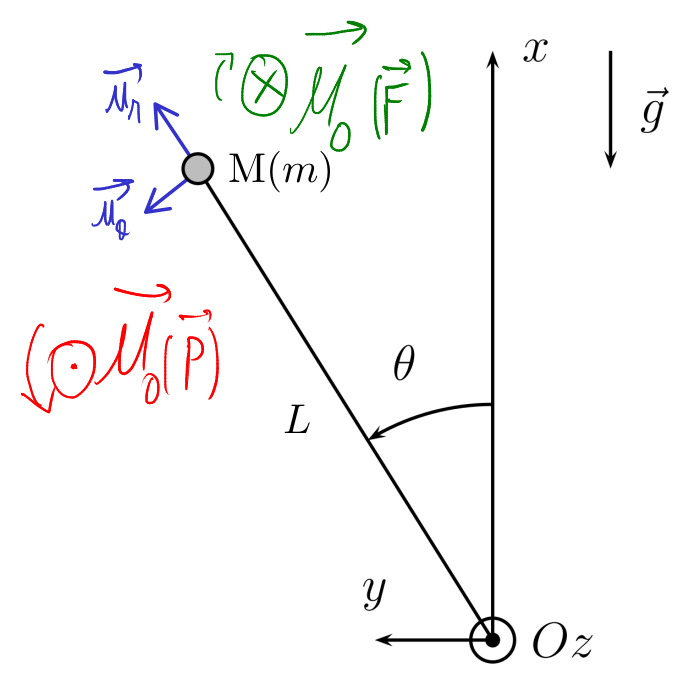
\includegraphics[width=5cm]{holweck_m}
		\end{center}
	\end{minipage}
	\hfill
	~
	\begin{itemize}
		\bitem{BDM}~:
		\vspace{-20pt}
		\begin{gather*}
			\left\{
			\begin{array}{ll}
				\Mcf_{\Or}(\Pf) & =
				\OM \wedge \Pf =
				mgL \ur \wedge (-\cos(\th)\ur+ \sin(\th)\ut) = mgL\sin(\th)\uz
				\\
				\Mcf_{\Or}(\Ff) & -C\th \uz
				\\
				\Lcf_{\Or}(\Mr) & =
				\OM \wedge m\vf =
				mL^2\tp \ur \wedge \ut = mL^2\tp \uz
			\end{array}
			\right.
			\\
			\beforetext{Ainsi}
			\boxed{\Mc_z(\Pf) = mgL\sin(\th)}
			\qquad
			\boxed{\Mc_z(\Ff) = -C\th}
			\qquad
			\boxed{\Lc_z(\Mr) = mL^2\tp}
		\end{gather*}
		\begin{align*}
			\beforetext{TMC $\Ra$}
			\dv{\Lc_z(\Mr)}{t}                                      & = \Mc_z(\Pf) + \Mc_z(\Ff)
			\\\Lra
			mL^2\tpp                                                & = mgL \sin(\th) - C\th
			\\\Lra
			\Aboxed{\tpp + \frac{C}{mL^2}\th - \frac{g}{L}\sin(\th) & = 0}
		\end{align*}
	\end{itemize}
}

\QR{%
	Pour $\th \ll 1$, linéariser le sinus pour obtenir une équation
	différentielle linéaire. À quelle condition entre $C$, $m$, $g$ et $L$, la
	solution à cette équation est-elle stable~?
}{%
	Autour de $\th\ind{eq} = 0$, $\sin(\th) \Sim_{\th \to 0} \th$. Ainsi,
	\begin{gather*}
		\tpp + \left( \frac{C}{mL^2} - \frac{g}{L} \right)\th = 0
		\Lra
		\boxed{\tpp + \w_0{}^2\th = 0}
		\\
		\beforetext{Équation caractéristique~:}
		r^2 + \w_0{}^2 = 0
		\Lra
		r^2 = -\w_0{}^2
		\\
		\beforetext{Stable $\Lra r \in \Cb \Ra$}
		\w_0{}^2 > 0
		\Lra
		\boxed{C > mgL}
	\end{gather*}
	Cette équation du second ordre a des solutions stable si et seulement si les
	racines de l'équation caractéristique sont complexes. En effet, avec $\th =
		A\exr^{rt}$, des racines réelles donnent des solutions divergentes~; seules
	les racines complexes donnent des solutions oscillantes en cosinus et sinus.
}

\QR{%
	Déterminer l'expression de la force du ressort spiral à partir de son moment.
	Établir alors l'expression de l'énergie potentielle totale du système, et
	retrouver la stabilité de la position d'équilibre $\th\ind{eq} = 0$.
}{%
	\begin{isd}
		\begin{DispWithArrows*}[fleqn, mathindent=0pt, groups]
			\Mcf_{\Or}(\Ff) &= \OM \wedge \Ff = -C\th\uz
			\\\Lra
			\ur \wedge \Ff &= -\frac{C}{L}\th\uz
			\Arrow{On déduit}
			\\\Ra
			\Aboxed{\Ff &= -\frac{C}{L}\th}
			\Arrow{Définition de $\Ec_{p,\rm el}$}
			\\
			\delta W(\Ff) &= -\dd{\Ec_{p,\rm el}}
			\Arrow{$\de W(\Ff) = \Ff \cdot \dd{\OM}$}
			\\\Lra
			\Ff \cdot \dd{\OM} &= -\dd{\Ec_{p,\rm el}}
			\Arrow{$
					\begin{array}{ll}
						\dd{\OM} & = \underbracket[1pt]{\dd{r}}_{r = L}\ur
						\\
						         & + L \dd{\th}\ut
					\end{array}
				$}
			\\\Lra
			\left( -\frac{C}{L}\th\ut \right) \cdot (L \dd{\th}\ut) &= -\dd{\Ec_{p,\rm
					el}}
			\\\Lra
			\dd{\Ec_{p,\rm el}} &= C\th \dd{\th}
			\CArrow{$\int \cdot$}
			\\\Ra
			\Aboxed{\Ec_{p,\rm el} &= \frac{1}{2}C\th^2 + K}
		\end{DispWithArrows*}
		\tcblower
		On remarque alors que l'énergie potentielle de ce ressort spiral a une
		expression similaire à celle du ressort linéaire $\Ec_{p,\rm el} = 1/2\,k
			x^2$
		\smallbreak
		On trouve l'énergie potentielle de pesanteur, en prenant la référence
		pour $\th = \frac{\pi}{2}$, $\boxed{\Ec_{p,p} = mgL \cos(\th)}$. Ainsi,
		\begin{align*}
			\Ec_{p,\rm tot}                                     & = mgL \cos(\th) + \frac{1}{2}C\th^2 + K
			\\\Ra
			\dv{\Ec_{p,\rm tot}}{\th}                           & = -mgL \sin(\th) + C\th
			\\\Ra
			\dv[2]{\Ec_{p,\rm tot}}{\th}                        & = -mgL \cos(\th) + C \underbracket[1pt]{>
				0}_{\mathclap{\text{si stable}}}
			\\
			\Ra
			\eval{\dv[2]{\Ec_{p,\rm tot}}{\th}}_{\th\ind{eq}=0} & = -mgL + C
			\\\Lra
			\Aboxed{C                                           & > mgl}
			\rlap{$\qquad\blacksquare$}
		\end{align*}
	\end{isd}
}

\QR{%
	À partir de l'équation différentielle simplifiée à la question 2,
	calculer la période $T$ des petites oscillations autour de $\th =
		0$.
}{%
	On reprend les résultats précédents~:
	\begin{gather*}
		\w_0 = \sqrt{\frac{C-mgL}{mL^2}} \Lra \frac{2\pi}{T_0}
		\\\Lra
		T_0 = 2\pi \sqrt{\frac{mL^2}{C-mgL}}
	\end{gather*}
}

\QR{%
	En posant $g_0 = C/mL$, déduire des résultats précédents une
	méthode de mesure de $g$.
}{%
	Il est logique de poser $g_0 = C/mL$, par analyse dimensionnelle de
	$\w_0{}^2$. En remplaçant dans $T_0$~:
	\begin{align*}
		T_0         & = 2\pi \sqrt{\frac{\cancel{mL}L}{mL(g_0-g)}}
		\\\Lra
		\Aboxed{T_0 & = 2\pi \sqrt{\frac{L}{g_0-g}}}
	\end{align*}
	On retrouve une expression proche de celle du pendule simple ($T_0 =
		\sqrt{\ell/g}$).
	\smallbreak
	Ainsi, en réglant $g_0 = C/mL$ à une valeur connue, si $g_0 > g$ on obtient
	des oscillations dont la période est directement reliée à $g_0 - g$. On
	pourrait penser à mesurer $g$ en réglant $g_0$ pour n'avoir aucune
	oscillation, mais la mesure de période est plus simple.
	\smallbreak
	On remarque cependant que quand $g > g_0$, d'après la question 1) on n'aura
	pas de solution stable mais des solutions en exponentielles divergentes, ce
	qui est une limite de cet outil.
}

\resetQ
\section{Pendule conique}

\enonce{%
	\noindent
	\begin{minipage}{0.70\linewidth}
		Dans un champ uniforme de pesanteur $\gf$ vertical et vers le bas, un point
		matériel M de masse $m$ tourne à la vitesse angulaire $\w$ constante autour
		de l'axe $(\Or z)$, dirigé vers le haut, et décrit ainsi un cercle de centre
		O et de rayon $R$. M est suspendue à un fil inextensible de longueur $L$ et
		de masse négligeable, fixé en un point A de $(\Or z)$. L'angle $\a$ de $(\Or
			z)$ avec AM est constant. \smallbreak On travaille dans le référentiel du
		laboratoire supposé galiléen. On utilisera le repère de la base cylindrique
		tel que $\OM = R\ur$.
	\end{minipage}
	\begin{minipage}{0.25\linewidth}
		\begin{center}
			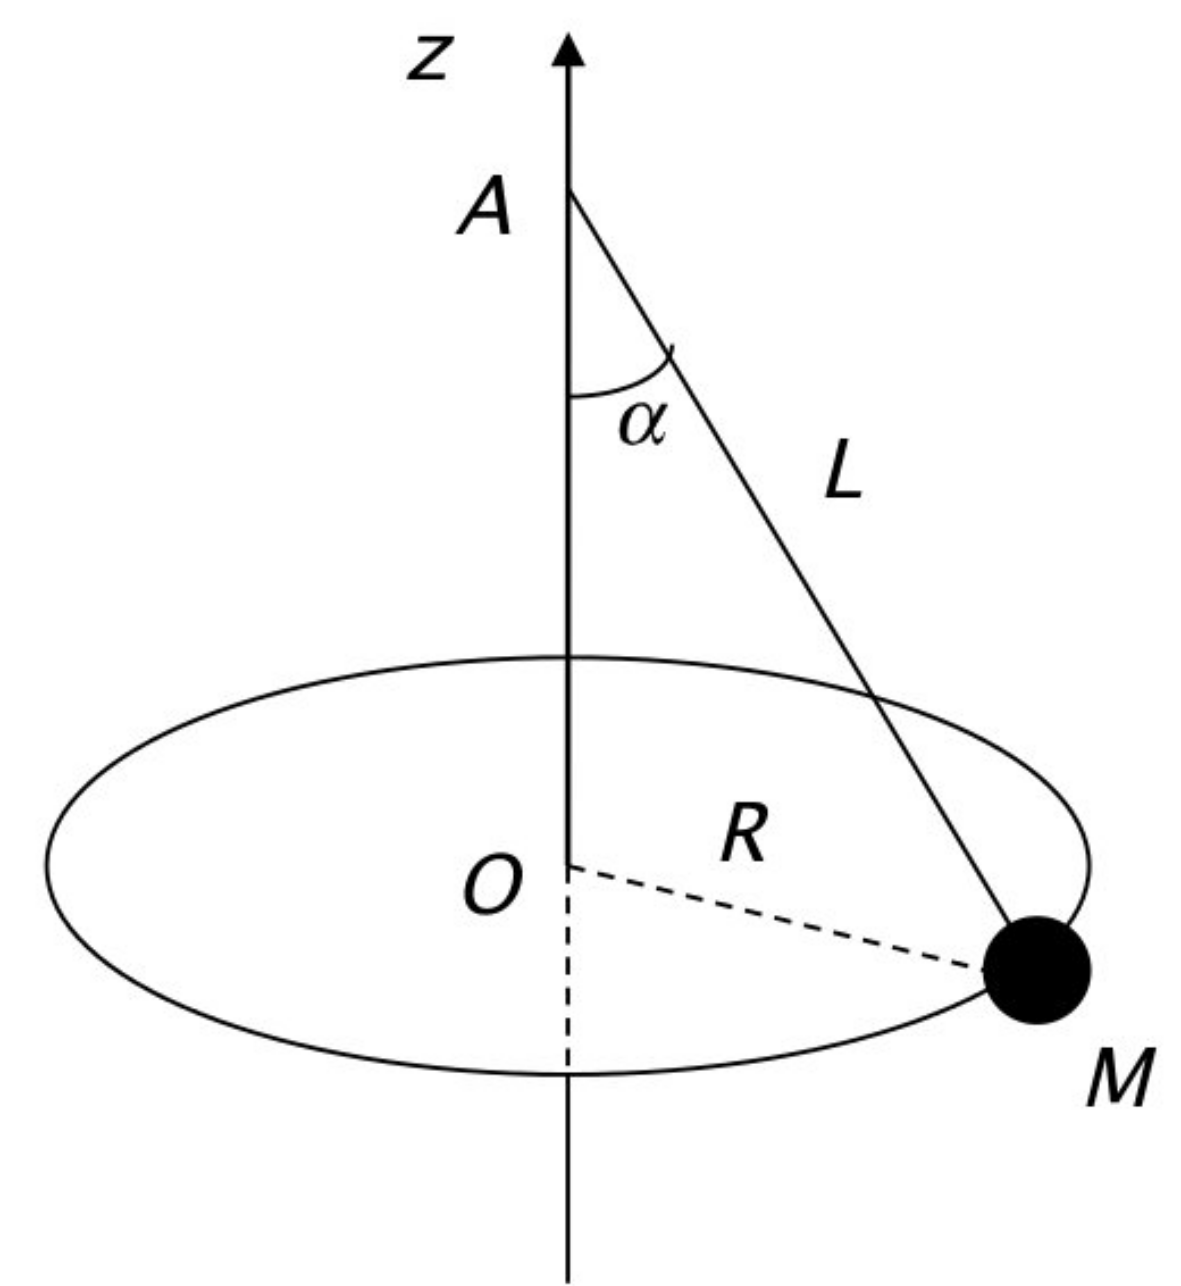
\includegraphics[width=\linewidth]{pendule_conique-plain}
		\end{center}
	\end{minipage}
}

\QR{%
	Exprimer le moment cinétique de M par rapport à A en fonction de $m$,
	$M$, $\w$ et $\a$.
}{%
	\noindent
	\begin{minipage}[t]{.50\linewidth}
		\begin{itemize}
			\bitem{Système}~: {masse}, repérée par M($m$).
			\bitem{Référentiel}~: terrestre supposé galiléen.
			\bitem{Repère}~: cylindrique $(\Or,\ur,\ut,\uz)$ (voir schéma).
			\bitem{Repèrage}~:
			\vspace{-20pt}
			\begin{align*}
				\OM & = R \ur = L \sin(\alpha) \ur       \\
				\vf & = R\tp\ut = L \w \sin(\alpha) \ut  \\
				\af & = R\tpp\ur = -L\w^2\sin(\alpha)\ur
			\end{align*}
      \bitem{Moment cinétique}~:
      Attention, on veut calculer le moment \textbf{par rapport à A}. Ainsi,
		\end{itemize}
	\end{minipage}
	\hfill
	\begin{minipage}[t]{.40\linewidth}
		\vspace{0pt}
		\begin{center}
			\includegraphics[width=5cm]{pendule_conique-corr}
		\end{center}
	\end{minipage}
	\vspace{-30pt}
	\begin{DispWithArrows*}
		\Lcf_{\Ar} &=
		\vvr{AM} \wedge \pf(\Mr) =
		\left( \vvr{AO} + \vvr{OM} \right) \wedge m\vf
		\Arrow{$\vvr{AM} = -L \cos(\alpha)\uz$}
		\\\Lra
		\Lcf_{\Ar} &=
		\left( -L \cos(\alpha)\uz + L\sin(\alpha)\ur \right)
		\wedge
		\left( mL\w \sin(\alpha)\ut \right)
		\Arrow{On distribue}
		\\\Lra
		\Lcf_{\Ar}(\Mr) &=
		-mL^2\w \sin(\alpha)\cos(\alpha) (-\ur) + mL^2\w \sin^2(\th)\uz
		\\\Lra
		\Aboxed{
			\Lcf_{\Ar}(\Mr) &=
			mL^2\w \left( \sin^2(\th)\uz + \sin(\alpha)\cos(\alpha) \ur \right)
		}
	\end{DispWithArrows*}
}

\QR{%
	Appliquer le TMC pour déduire $\cos\a$ en fonction de $g$, $L$ et
	$\w$.
}{%
	\vspace{-15pt}
	\begin{itemize}
		\bitem{BDF}~:
		\vspace{-10pt}
		\[
			\left\{
			\begin{array}{ll}
				\Pf & = -mg \uz
				\\
				\Tf & = -T \frac{\vvr{AM}}{\norm{\vvr{AM}}}
				\qou
				\Tf = T (\cos(\alpha)\uz - \sin(\alpha)\ur)
				\quad \text{mais inutile}
			\end{array}
			\right.
		\]
		\bitem{BDM}~:
		\vspace{-20pt}
		\begin{gather*}
			\left\{
			\begin{array}{ll}
				\Mcf_{\Ar}(\Pf) & =
				\vvr{AM} \wedge \Pf =
				L(\sin(\alpha)\ur - \cos(\alpha)\uz) \wedge (-mg \uz)
				\Lra
				\Mcf_{\Ar}(\Pf) = +mgL \sin(\alpha)\ut
				\\
				\Mcf_{\Ar}(\Tf) & = \vvr{AM} \wedge \Tf = \of
			\end{array}
			\right.
		\end{gather*}
		\bitem{TMC}~:
		\vspace{-15pt}
		\begin{DispWithArrows*}[groups]
			\dv{\Lcf_{\Ar}(\Mr)}{t} &= \sum_{i} \Mcf_{\Ar}(\Ff) = \Mcf_{\Ar}(\Pf)
			\\\Lra
			mL^2\w \left(
			\sin^2(\alpha) \underbracket[1pt]{\dv{\uz}{t}}_{=0} +
			\sin(\alpha)\cos(\alpha) \underbracket{\dv{\ur}{t}}_{=\w \ut}
			\right) &= mgL \sin(\alpha) \ut
			\CArrow{$\cdot \ut$}
			\\\Ra
			\cancel{m}L^{\bcancel{2}}\w^2\dcancel{\sin(\alpha)} \cos(\alpha) &=
			\cancel{m}g \bcancel{L}\dcancel{\sin(\alpha)}
			\\\Lra
			\Aboxed{\cos(\alpha) &= \frac{g}{L\w^2}}
		\end{DispWithArrows*}
	\end{itemize}
}

\QR{%
	Retrouver ce résultat à partir du PFD.
}{%
	\vspace{-15pt}
	\begin{gather*}
		\beforetext{PFD~:}
		\dv{\pf}{t} = \sum_i \Ff_i
		\\\Lra
		-mL\w^2\sin(\alpha)\ur = -mg\uz + T(\cos(\alpha)\uz - \sin(\alpha)\ur)
		\\\Lra
		\left\{
		\begin{array}{ll}
			-mL\w^2\sin(\alpha) & -T \sin(\alpha)
			\\
			0                   & = -mg + T\cos(\alpha)
		\end{array}
		\right.
		\Lra
		\left\{
		\begin{array}{ll}
			T & mL\w^2
			\\
			T & = \frac{mg}{\cos(\alpha)}
		\end{array}
		\right.
		\\\Lra
		\boxed{\cos(\alpha) = \frac{g}{L\w^2}}
		\rlap{$\qquad\blacksquare$}
	\end{gather*}
}

\resetQ
\section{Frottements d'un satellite}
\enonce{%
	Un satellite S de masse $m$ décrit une trajectoire circulaire uniforme
	d'altitude $h_0$ autour de la Terre de masse $m_T$ et de rayon $R_T$, dans le
	référentiel géocentrique.
}

\QR{%
	Exprimer la norme $v$ de son vecteur vitesse et son énergie mécanique
	$\Ec_m$ en fonction de $\Gc$, $m_T$, $m$, $R_T$ et $h_0$. On pourra
	localement introduire $R=R_T+h_0$.
}{%
	\noindent
	\begin{minipage}[t]{0.70\linewidth}
		\begin{enumerate}[label=\sqenumi]
			\bitem{Système}~: \{satellite\} point matériel M de masse $m$
			\bitem{Référentiel}~: géocentrique, supposé galiléen.
			\bitem{Repère}~:
			polaire $(\Or,\ur,\ut)$ avec O centre du Soleil, R le
			rayon supposé constant ($\dot{R} = 0$).
			\bitem{Repérage}~:
			\vspace{-15pt}
			\begin{align*}
				\OM & = (R_{\Ter}+h_0)\ur = R \ur               \\
				\vf & = R\tp\ut  \quad \Ra \quad v = \abs{R\tp} \\
				\af & = -R\tp^2\ur + R\tpp\ut
			\end{align*}
			\bitem{Bilan des forces}~:
			$\DS\Ff_g = -\Gc \frac{mM_{\Ter}}{R^2}\ur \Ra \Ec_p = -\Gc
				\frac{mM_{\Ter}}{R}$.
		\end{enumerate}
	\end{minipage}
	\hfill
	\begin{minipage}[t]{0.25\linewidth}
		~\vspace*{-20pt}
		\begin{center}
			\includegraphics[width=\linewidth]{frott_corra.pdf}
			\captionsetup{justification=centering}
			\captionof{figure}{\\Orbite circulaire.}
		\end{center}
	\end{minipage}
	\begin{enumerate}[label=\sqenumi, start=6]
		\bitem{PFD}~:
	\end{enumerate}
	\begin{isd}[righthand ratio=.4]
		\begin{DispWithArrows}< m\af = \Ff_{g} \Lra >
			-mR\tp^2 &= -\Gc \frac{mM_{\Ter}}{R^2}\ur
			\Lra
			\tp = \sqrt{\frac{\Gc M_{\Ter}}{R^3}}
			\label{eq:ivc71}
			\\
			mR\tpp &= 0
			\Lra
			\tp = \cte
			\label{eq:ivc72}
		\end{DispWithArrows}
		\eqref{eq:ivc71} donne alors
		\begin{equation}
			\boxed{v = \sqrt{\frac{\Gc M{_\Sr}}{R_{\Ter}+h_0}}}
			\rlap{$\qquad\blacksquare$}
			\label{eq:ivc73}
		\end{equation}
		\tcblower
		Enfin, avec~\eqref{eq:ivc73} et l'énergie mécanique, on a
		\begin{DispWithArrows*}[fleqn, mathindent=0pt]
			\Ec_m         & =
			\frac{1}{2}mR^2\tp^2 - \Gc\frac{mM{_\Sr}}{R}
			\Arrow{$R\tp = \sqrt{\frac{\Gc M{_\Sr}}{R}}$}
			\\\Lra
			\Ec_m         & = \frac{1}{2}m\frac{\Gc M{_\Sr}}{R} - \Gc\frac{mM{_\Sr}}{R}
			\\\Lra
			\Aboxed{\Ec_m & = -\frac{1}{2}\Gc\frac{mM{_\Sr}}{R_{\Ter}+h_0}}
			\qed
		\end{DispWithArrows*}
	\end{isd}
}

\begin{blocQR}
	\item
	Le satellite étant sur une orbite basse, il subit de la part des
	hautes couches de l'atmosphère une force de frottements qui modifie son
	altitude $h$. Cependant, \textbf{on considère que la trajectoire sur un
		tour reste quasi-circulaire}~; ainsi les expressions précédentes restent
	valables en remplaçant $h_0$ par $h(t)$.
	\QR{%
		Le travail des forces de frottements est-il moteur ou
		résistant~? En déduire le signe de $\dv{\Ec_m}{t}$.
	}{%
		Les forces de frottements sont toujours résistantes. En effet,
		\begin{gather*}
			\Ff_f = -\alpha\vf
			\qdc
			\Pc(\Ff_f) = -\alpha v^2 < 0
			\\
			\beforetext{D'où par TPM}
			\boxed{\dv{\Ec_m}{t} = \Pc(\Ff_f) < 0}
		\end{gather*}
	}

	\QR{%
		Comment évolue le rayon de l'orbite du satellite au cours du
		temps~? Tracer l'allure de sa trajectoire.
	}{%
		\noindent
		\begin{minipage}[]{.75\linewidth}
			$r(t)$ diminue forcément, puisque
			\[
				\Ec_m = -\frac{k}{R_{\Ter}+h(t)} \searrow \qMath{quand} h\searrow
			\]
			\textbf{Attention}, $\Ec_m < 0$ donc $\abs{\Ec_m} \nearrow$ quand $h
				\searrow$ mais on a bien $\Ec_m \searrow$.
		\end{minipage}
		\hfill
		\begin{minipage}[]{.20\linewidth}
			~
			\begin{center}
				\includegraphics[width=\linewidth]{frott_corrb}
			\end{center}
		\end{minipage}
	}

	\QR{%
		En déduire le sens de variation de la vitesse. Commenter.
	}{%
		\[
			v = \sqrt{\frac{\Gc m M_{\Ter}}{R_{\Ter}+h(t)}}
			\qdc
			\boxed{v \nearrow \qMath{quand} h\searrow}
		\]
		Peu intuitif \textit{a priori} car les frottements sont censés réduire la
		vitesse, mais en réalité les frottements réduisent surtout l'énergie totale
		d'un corps. À la surface de la Terre sur un sol plat, les frottements ne
		font que perdre de l'énergie cinétique, mais ici réduire l'énergie mécanique
		réduit le rayon, et la vitesse doit augmenter en vertu de la 3\ieme{} loi
		de \textsc{Kepler}.
	}

\end{blocQR}

\resetQ
\section{Comète de \textsc{Halley}}

\enonce{%
	\noindent
	\begin{minipage}{0.70\linewidth}
		La comète de \textsc{Halley} est la plus connue. La première mention de son
		observation date de 611 av. J.-C.\ en Chine, et on la retrouve tout au long
		de l'Antiquité et du Moyen Âge, évidemment sans savoir qu'il s'agit d'une
		seule comète. Cette découverte a été formalisée en 1705 par Edmond
		\textsc{Halley,} qui publia un livre avançant que les observations en 1531,
		1607 et 1682 concernaient en fait la même comète. Son prochain passage est
		prévu en 2061. On sait aujourd'hui que la comète de \textsc{Halley} suit une
		trajectoire elliptique de période de révolution autour du Soleil 76 ans, sa
		distance minimale au Soleil étant de $d_{\min} = \SI{0.59}{UA}$.
	\end{minipage}
	\hfill
	\begin{minipage}{.25\linewidth}
		\begin{center}
			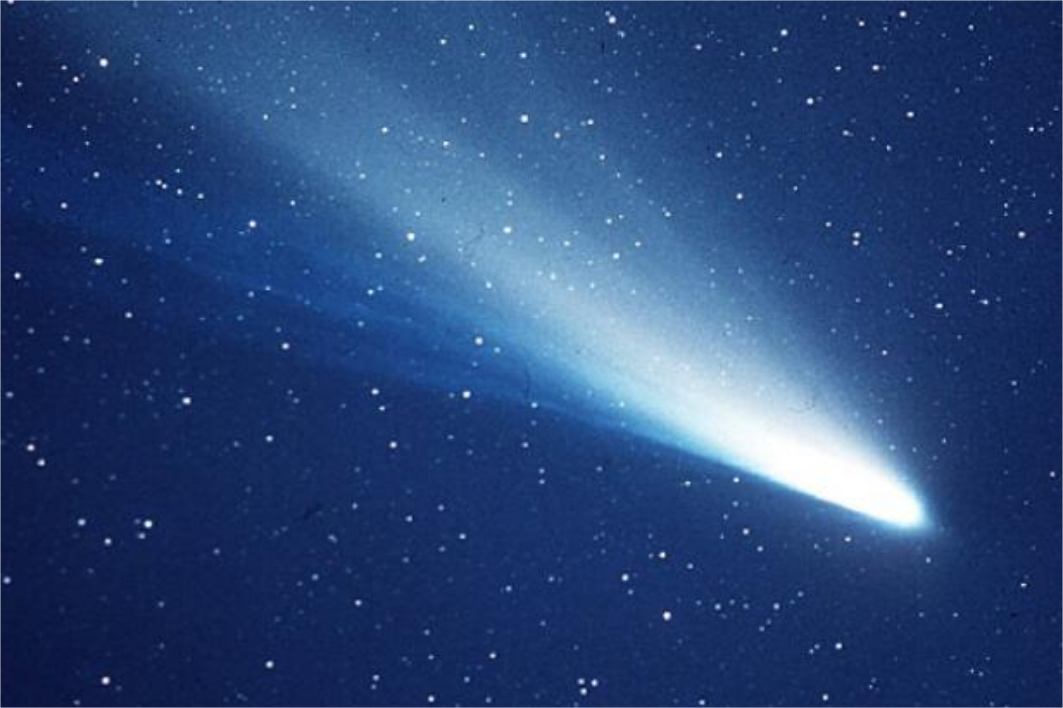
\includegraphics[width=\linewidth]{halley}
		\end{center}
	\end{minipage}
	\begin{tcb}(defi)<lft>'l'{Données}
		\begin{itemize}
			\item Masse solaire $M{_\Sr} = \SI{2.0e30}{kg}$.
			\item UA signifie «~unité astronomique~», et correspond à la distance
			      moyenne entre la Terre et le Soleil. $\SI{1}{UA} = \SI{1.5e11}{m}$.
		\end{itemize}
	\end{tcb}
}

\QR{%
	Faire un schéma de la trajectoire de la comète en faisant aussi
	apparaître la position du Soleil et $d_{\min}$.
}{%
	~
	\begin{center}
		\includegraphics[width=.35\linewidth]{halley_corra}
	\end{center}
}

\QR{%
	Déduire de la troisième loi de \textsc{Kepler} la plus grande distance
	de la comète au Soleil.
}{%
	On trouve vite
	\[
		d_{\max} + d_{\min} = 2a
		\Lra
		d_{\max} = 2a - d_{\min}
	\]
	Deux méthodes pour les unités~:
	\smallbreak
	\begin{isd}[sidebyside align=top]
		\tcbsubtitle{\fatbox{\textbf{Tout en SI}}}
		\begin{gather*}
			\beforetext{Or,}
			\frac{T_{\Hr}^2}{a_{\Hr}^3} = \frac{4\pi^2}{\Gc M_{\Sr}}
			\Lra
			\boxed{a_{\Hr} = \sqrt{\frac{\Gc M_{\Sr}}{4\pi^2}T_{\Hr}^2}}
			\\
			\qav
			\left\{
			\begin{array}{rcl}
				\Gc     & = & \SI{6.67e-11}{SI}
				\\
				M_{\Sr} & = & \SI{2.0e30}{kg}
				\\
				T_{\Hr} & = & \SI{76}{ans} = \SI{2.40e40}{s}
			\end{array}
			\right.\\
			\AN
			\xul{
				a_{\Hr} = \SI{2.69e12}{m} = \SI{17.9}{UA}
			}
		\end{gather*}
		\tcblower
		\tcbsubtitle{\fatbox{\textbf{En unités astronomiques}}}
		\begin{gather*}
			\frac{T_{\Hr}^2}{a_{\Hr}^3} = \frac{T_{\Ter}^2}{a_{\Ter}^3}
			\Lra
			\boxed{
			a_{\Hr} = a_{\Ter} \left( \frac{T_{\Hr}}{T_{\Ter}} \right)^{\frac{3}{2}}
			}
			\\
			\AN
			\xul{
				a_{\Hr} = \SI{17.9}{UA}
			}
			\qav
			\left\{
			\begin{array}{rcl}
				T_{\Hr}  & = & \SI{76}{ans}
				\\
				a_{\Ter} & = & \SI{1}{UA}
				\\
				T_{\Ter} & = & \SI{1}{an}
			\end{array}
			\right.
		\end{gather*}
	\end{isd}
	\begin{gather*}
		\beforetext{Dans tous les cas,}
		d_{\max} = 2a - d_{\min}
		\qav
		\left\{
		\begin{array}{rcl}
			a        & = & \SI{17.9}{UA}
			\\
			d_{\min} & = & \SI{0.59}{UA}
		\end{array}
		\right.\\
		\AN
		\xul{
			d_{\max} = \SI{35.3}{UA}
		}
	\end{gather*}
}

\QR{%
	Une conique est décrite par une équation polaire de la forme
	\[r(\th) = \frac{p}{1-e\cos\th}\]
	où l'origine du repérage polaire est prise sur un des foyers de la
	conique. Déterminer le paramètre $p$ et l'excentricité $e$ de la
	trajectoire de la comète de \textsc{Halley}.
}{%
	\noindent
	\begin{minipage}[]{.60\linewidth}
		On décrit $d_{\min}$ et $d_{\max}$ avec $r(\th)$ grâce à un schéma~:
		\begin{gather*}
			\left\{
			\begin{aligned}
				d_{\min} & = r(0) = \frac{p}{1-e}
				\\
				d_{\max} & = r(\pi) = \frac{p}{1+e}
			\end{aligned}
			\right.
			\Lra
			\left\{
			\begin{aligned}
				1-e & = r(0) = \frac{p}{d_{\min}}
				\qquad (1)
				\\
				1+e & = r(\pi) = \frac{p}{d_{\max}}
				\qquad (2)
			\end{aligned}
			\right.
		\end{gather*}
	\end{minipage}
	\hfill
	\begin{minipage}[c]{.35\linewidth}
		~
		\begin{center}
			\includegraphics[width=\linewidth]{halley_corrb}
		\end{center}
	\end{minipage}
	\begin{isd}
		\vspace{-15pt}
		\begin{align*}
			\beforetext{$(1) + (2) \Ra $}
			                            &
			\\
			1-\cancel{e} + 1+\cancel{e} & =
			p \left( \frac{1}{d_{\min}} + \frac{1}{d_{\max}} \right)
			\\\Lra
			2                           & = p \left( \frac{d_{\max}+d_{\min}}{d_{\min}d_{\max}} \right)
			\\\Lra
			\Aboxed{p                   & = 2 \frac{d_{\min}d_{\max}}{d_{\min}+d_{\max}}}
		\end{align*}
		\tcblower
		\vspace{-15pt}
		\begin{align*}
			\beforetext{$(2) - (1) \Ra$}
			                              &
			\\
			\cancel{1}+e - (\cancel{1}-e) & =
			p \left( \frac{1}{d_{\max}}- \frac{1}{d_{\min}} \right)
			\\\Lra
			\cancel{2}e                   & =
			\cancel{2}
			\frac{\bcancel{d_{\min}d_{\max}}}{d_{\min}+d_{\max}}
			\left( \frac{d_{\min}-d_{\max}}{\bcancel{d_{\min}d_{\max}}} \right)
			\\\Lra
			\Aboxed{e                     & = \frac{d_{\min}-d_{\max}}{d_{\min}+d_{\max}}}
		\end{align*}
	\end{isd}
}

\resetQ
\section{Changement d'orbite}

\enonce{%
	\noindent
	\begin{minipage}{0.70\linewidth}
		Un satellite artificiel assimilé à un point matériel M de masse $m$ trouve
		sur une orbite circulaire provisoire de rayon $r_1 = \SI{7500}{km}$ autour
		de la Terre. On souhaite le faire passer sur son orbite définitive de rayon
		$r_2 = \SI{42200}{km}$ (orbite géostationnaire).
		\smallbreak
		Pour cela, on le fait d'abord passer sur une orbite de transfert elliptique
		dont le périgée P est à la distance $r_1$ et l'apogée A à la distance $r_2$ du
		centre O de la Terre. Dès que le satellite arrive en A, on le fait passer sur
		l'orbite circulaire de rayon $r_2$.
		\smallbreak
		Ces deux changements d'orbite sont obtenus par allumage d'un moteur placé sur
		le satellite~: ce processus est très bref (par rapport aux périodes
		orbitales), donc on considérera que la vitesse passe instantanément de $v_1$ à
		$v_{e1}$ en P, puis de $v_{e2}$ à $v_2$ en A (sans changer de direction dans
		les deux cas).
	\end{minipage}
	\hfill
	\begin{minipage}{0.25\linewidth}
		\begin{center}
			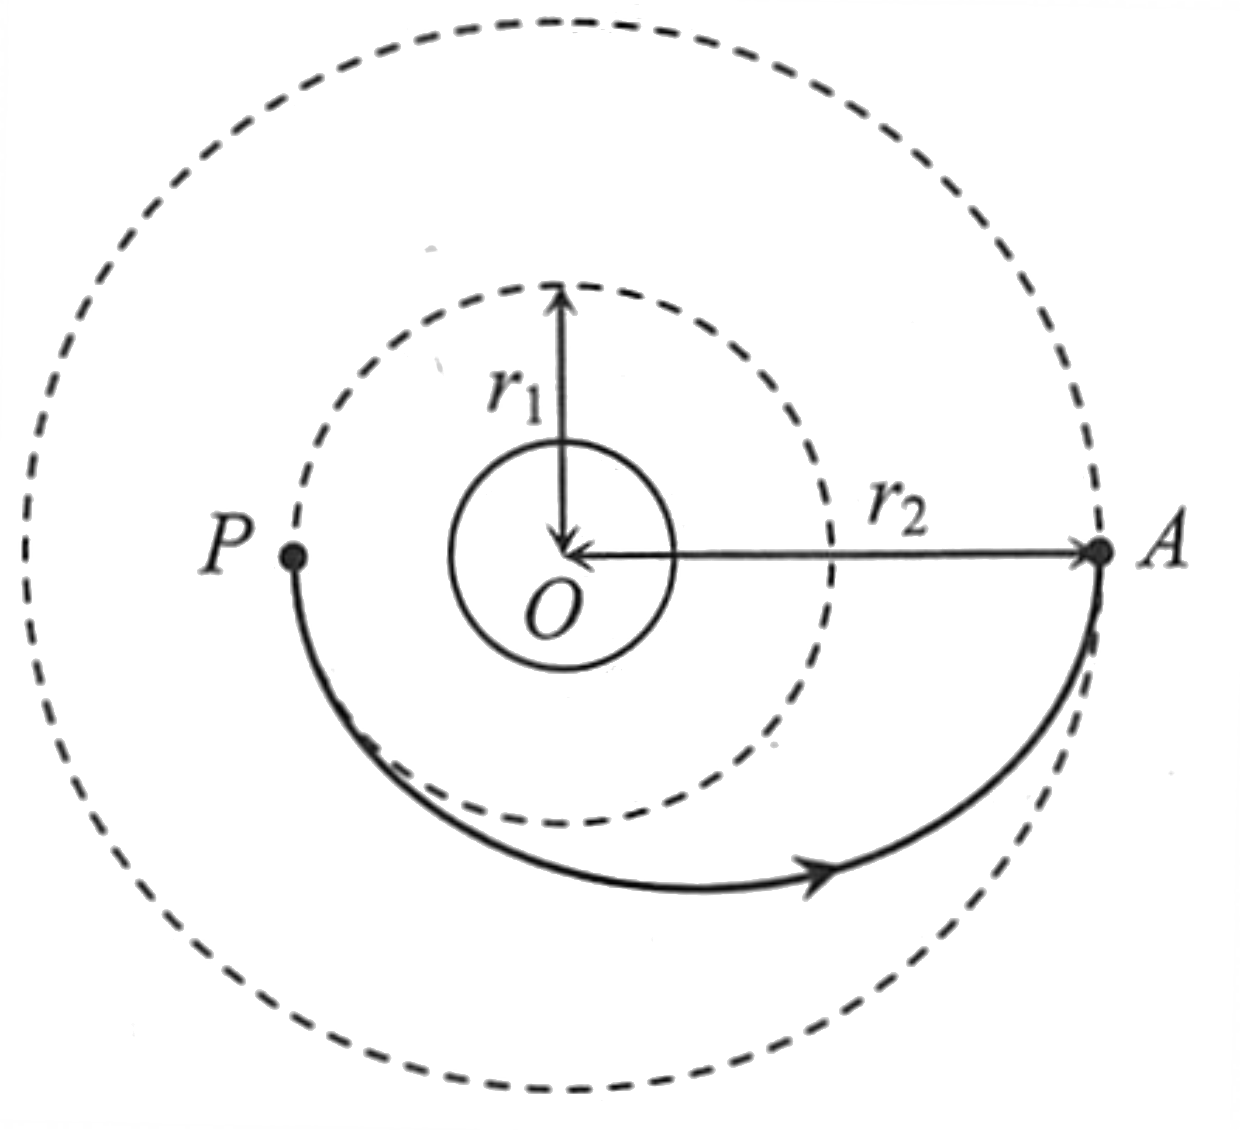
\includegraphics[width=\linewidth]{chgmt_orbite-plain_white}
		\end{center}
	\end{minipage}
	\begin{tcb}(defi)<lft>'l'{Données}
		$M_{\rm Terre} = \SI{5.97e24}{kg}$~; $\Gc = \SI{6.67e-11}{SI}$~: $m =
			\SI{1000}{kg}$.
	\end{tcb}
}

\QR{%
	Calculer la vitesse $v_1$.
}{%
	Sur une orbite circulaire, la vitesse est uniforme et on a $v_{1} = r_1\tp_1$.
	Avec le PFD usuel, on trouve
	\begin{gather*}
		\tp_1 = \sqrt{\frac{\Gc M}{r_1{}^3}}
		\Ra
		\boxed{v_1 = \sqrt{\frac{\Gc M}{r_1}}}
		\Ra
		\xul{v_1 = \SI{7300}{m.s^{-1}}}
	\end{gather*}
}

\QR{%
	Donner l'expression de l'énergie mécanique du satellite sur chacune
	des trois orbites, en fonction de $r_1$ et $r_2$.
}{%
	Ici aussi calcul classique~:
	\begin{gather*}
		\Ec_{m,i} =
		\frac{1}{2}mv_{i}{}^2 - \frac{\Gc Mm}{r_i} =
		\frac{1}{2}\frac{\Gc Mm}{r_i} - \frac{\Gc Mm}{r_i}
		\\
		\beforetext{D'où}
		\boxed{\Ec_{m,1} = -\frac{\Gc Mm}{2r_1}}
		\qet
		\boxed{\Ec_{m,2} = -\frac{\Gc Mm}{2r_2}}
	\end{gather*}
	Pour l'orbite elliptique, on remplace $r$ par $a$. Or, on relie $a$ au rayon
	$r_{\rm P}$ et $r_{\Ar}$ par la définition du grand axe, et on identifie
	$r_{\rm P}$ à $r_1$ et $r_{\Ar}$ à $r_2$~:
	\begin{gather*}
		2a = r_{\rm P} + r_{\Ar} = r_1 + r_2
		\\\Ra
		\boxed{\Ec_{m,e} = - \Gc \frac{Mm}{r_1+r_2}}
	\end{gather*}
}

\QR{%
	Calculer la vitesse $v_{e1}$ après le premier transfert, et la
	variation $\D v_{\rm P} = v_{e1}-v_1$. Calculer également le travail $W_{\rm P}$
	fourni par le moteur au satellite en ce point.
}{%
	Le changement de vitesse instantané suppose que la position est fixe et que
	l'énergie potentielle reste donc constante pour passer de $v_1$ à $v_{e1}$.
	Ainsi, l'allumage du réacteur ne fait changer que la vitesse, et on a
	\begin{align*}
		\Delta_{1,e}\Ec_m                                       & = \Ec_{m,e} - \Ec_{m,1}
		\\\Lra
		-\Gc Mm \left( \frac{1}{r_1+r_2}-\frac{1}{2r_1} \right) & =
		\frac{1}{2}m v_{e1}^2 - \frac{1}{2}mv_{1}^2
		\\\Lra
		\frac{1}{2}mv_{e1}^2                                    & =
		-\Gc Mm \left( \frac{\cancel{2}r_1 - \cancel{r_1} - r_2}{2r_1(r_1+r_2)}
		\right) + \Gc \frac{Mm}{2r_1} {\color{orange} \times \frac{r_1+r_2}{r_1+r_2}}
		\\\Lra
		\frac{1}{2}\cancel{m}v_{e1}^2                           & = \frac{\Gc M\cancel{m}}{\dcancel{2}r_1(r_1+r_2)}
		\underbracket[1pt]{\left( \bcancel{r_1}+r_2 - (\bcancel{r_1} - r_2)
			\right)}_{=\dcancel{2}r_2}
		\\\Lra
		\Aboxed{v_{e1}                                          & = \sqrt{\frac{2 \Gc Mr_2}{r_1(r_1+r_2)}}}
		\Lra
		\xul{v_{e1} = \SI{9520}{m.s^{-1}}}
		\\\Ra
		\Delta v_{\rm P}                                        & = \SI{2220}{m.s^{-1}}
		\\
		\beforetext{TEM~:}
		\Delta_{1,e}\Ec_m                                       & = \Delta_{1,e}W(\Ff\ind{mot}) = W_{\rm P}
		\\\Lra
		\Aboxed{W_{\rm P}                                       & = \frac{\Gc Mm(r_2-r_1)}{2r_1(r_1+r_2)}}
		\Lra
		\xul{W_{\rm P} = \SI{19}{GJ}}
	\end{align*}
}

\QR{%
	Déterminer une relation entre $v_{e1}$, $v_{e2}$, $r_1$ et $r_2$.
	Calculer $v_{e2}$.
}{%
	Relier des vitesses et des rayons ensemble sur deux parties de la trajectoire
	laisse penser qu'on cherche à trouver une constante du mouvement permettant de
	relier ces grandeurs entre elles à deux instants. On a déjà utilisé le
	théorème de l'énergie mécanique, on doit chercher une autre grandeur
	conservée.
	\smallbreak
	La plus évidente est le moment cinétique, et en effet aux points P et A
	l'expression du moment cinétique est simple, puisqu'on y a $\rp_{P|A} = 0$~:
	\begin{align*}
		\Lcf_{\Or}({\rm P)}              & =
		\vvr{OP} \wedge m\vf_{\rm P} =
		r_1 \ur \wedge mv_{e1}\ut = mr_1v_{e1}\uz
		\\
		\Lcf_{\Or}({\rm A)}              & =
		\vvr{OA} \wedge m\vf_{\rm A} =
		mr_2v_{e2}\uz
		\\
		\beforetext{Or $\dv{\Lcf_{\Or}}{t}=\of \Ra $}
		\cancel{m}r_1v_{e1}\bcancel{\uz} & = \cancel{m}r_2v_{e2}\bcancel{\uz}
		\\\Lra
		\Aboxed{r_1v_{e1}                & = r_2v_{e2}}
		\\
		\beforetext{Ainsi}
		\Aboxed{v_{e2}                   & = v_{e1} \frac{r_1}{r_2} =
			\sqrt{\frac{2 \Gc Mr_1}{r_2(r_1+r_2)}}}
		\\
		v_{e2}                           & = \SI{1690}{m.s^{-1}}
	\end{align*}

}

\QR{%
	Calculer la variation de vitesse $\D v_A = v_2 - v_{e2}$ lors du
	second transfert, ainsi que le travail $W_A$ fourni par le moteur au
	satellite.
}{%
	On reprend $v_2$ avec la première question, et on calcule la différence de
	vitesse avec la dernière~:
	\begin{gather*}
		v_2 = \sqrt{\frac{\Gc M}{r_2}} = \SI{3080}{m.s^{-1}}
		\\\Ra
		\boxed{\Delta{v_{\Ar}} = \SI{1390}{m.s^{-1}}}
		\beforetext{De plus,}
		\Delta_{e,2}\Ec_m = W_{\Ar}
		\Lra
		W_{\Ar} = - \frac{\Gc Mm}{2r_2} + \frac{\Gc Mm}{r_1+r_2}
		\\\Lra
		\boxed{W_{\Ar} = \frac{\Gc Mm(r_2-r_1)}{2r_2(r_1+r_2)}}
		\Lra
		\xul{W_{\Ar} = \SI{3.3}{GJ}}
	\end{gather*}
	On sait que la vitesse diminue quand $r$ augmente (3\ieme{} loi), donc $W
		\searrow$ de P à A~: c'est bien logique.
}

\resetQ
\section{Alerte à l'astéroïde~!}
\enonce{%
	\noindent
	\begin{minipage}[c]{.45\linewidth}
		~
		\begin{center}
			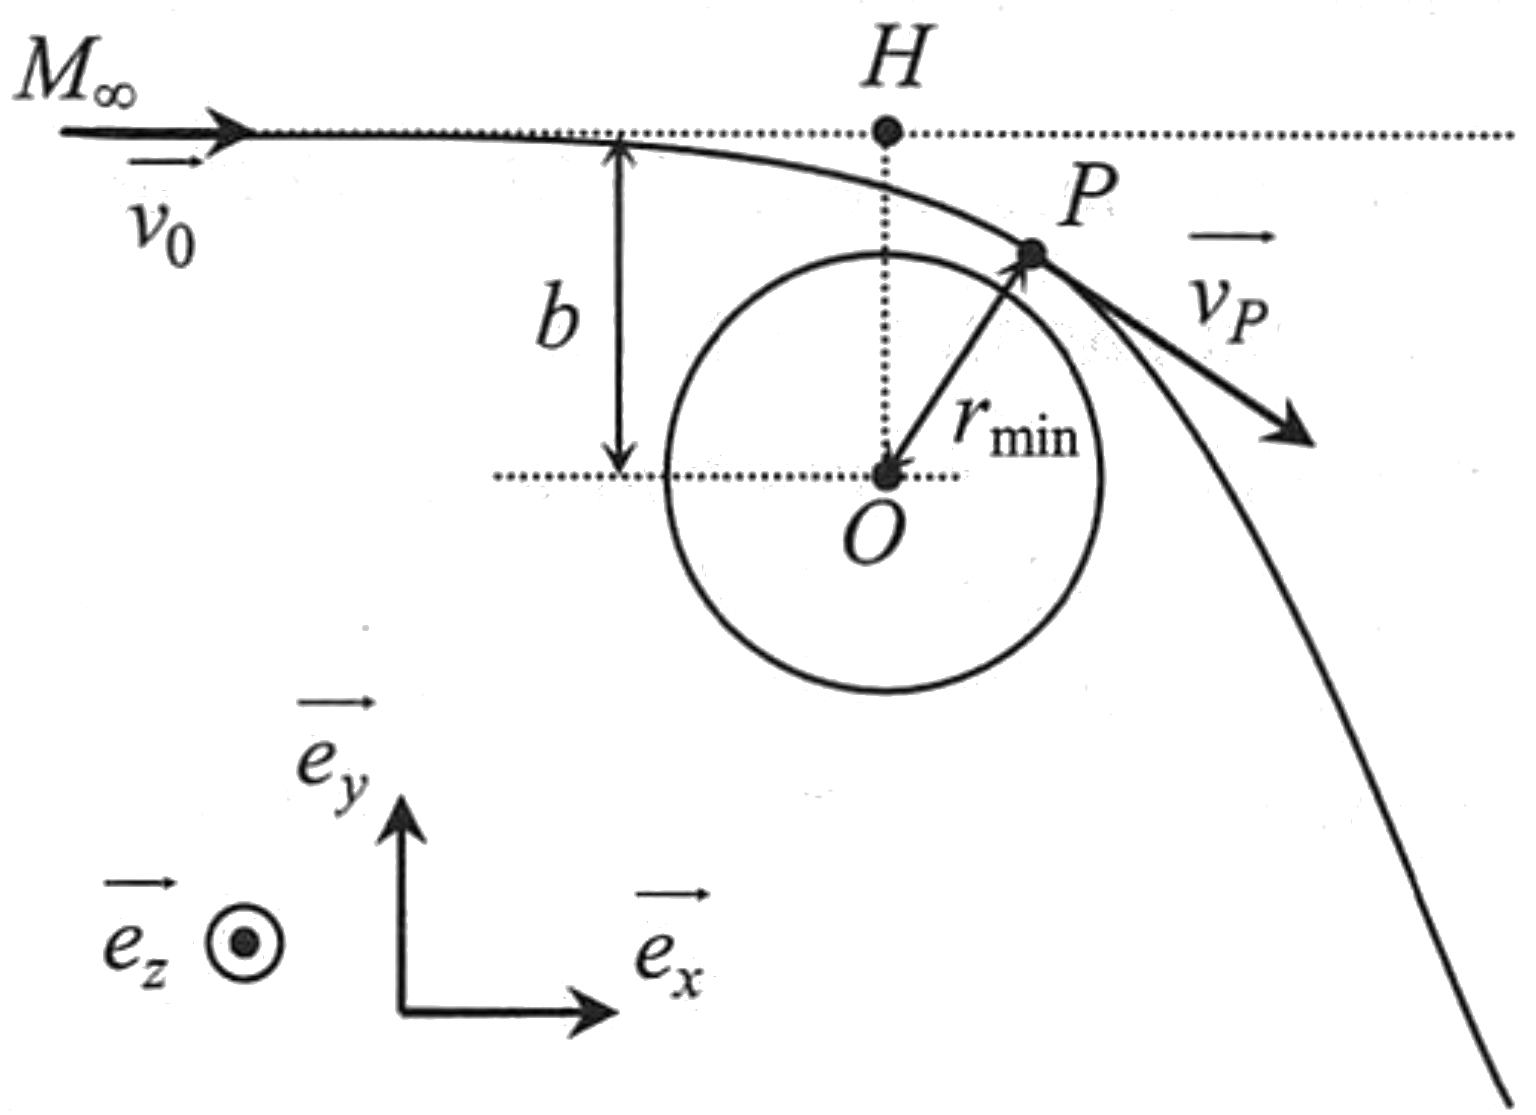
\includegraphics[width=\linewidth]{alerte_aste-plain_white}
			\captionof{figure}{Trajectoire de l'astéroïde.}
			\label{fig:aste}
		\end{center}
	\end{minipage}
	\hfill
	\begin{minipage}[c]{.50\linewidth}
		De nombreux objets, dits géocroiseurs, passent à proximité de la Terre… et
		parfois la heurtent~!
		\smallbreak
		On considère ici un astéroïde de masse $m$ actuellement très éloigné de la
		Terre et de tout autre astre. Il a donc un vecteur vitesse $\vfo$ constant. Le
		prolongement de sa trajectoire rectiligne passe à une distance $b$ (appelée
		paramètre d'impact) du centre O de la Terre.
		\smallbreak
		Cependant lorsqu'il se rapprochera de la Terre, l'attraction gravitationnelle
		de celle-ci va dévier l'astéroïde selon une trajectoire hyperbolique. On
		appelle périgée le point P de cette trajectoire le point le plus proche du
		centre de la Terre.
	\end{minipage}
}

\QR{%
	Quelles sont les deux grandeurs dynamiques de l'astéroïde qui se conservent
	au cours de son mouvement~? Traduire en équation leurs conservations entre les
	deux position $\Mr_{\infty}$ et P.
}{%
	\ifprof{\vspace{-15pt}}
	\begin{itemize}
		\bitem{Énergie mécanique}~:
		\[
			\Ec_m = \Ec_c + \Ec_p = \frac{1}{2}mv^2 - \Gc \frac{Mm}{r} = \cte
		\]
		\begin{itemize}
			\item Lorsqu'il est très éloigné ($\Mr_{\infty}$), $v=v_0$ et $r\to\infty$
			      donc l'énergie potentielle est nulle et $\Ec_m = \frac{1}{2}mv_0{}^2$.
			\item Au périgée P, $\Ec_m = \frac{1}{2}mv\ind{P}{}^2 - \Gc
				      \frac{Mm}{r_{\min}}$.
		\end{itemize}
		\begin{gather}
			\beforetext{Ainsi,}
			\boxed{\frac{1}{2}mv_0{}^2 = \frac{1}{2}mv\ind{P}{}^2 - \Gc
			\frac{Mm}{r_{\min}}}
			\label{eq:alerte1}
		\end{gather}
		\bitem{Moment cinétique}~: $\Lcf_{\Or}(\Mr_{\infty}) = \Lcf_{\Or}({\rm P})$
		d'où
		\begin{align}
			\vvr{OM_{\infty}} \wedge \cancel{m}\vfo^2               & =
			\vvr{OP} \wedge \cancel{m} \vf\ind{P}
			\nonumber
			\\\Lra
			\left( \vvr{OH} + \vvr{HM_{\infty}} \right) \wedge \vfo & =
			\vvr{OP} \wedge \vf\ind{P}
			\nonumber
			\\\Lra
			-bv_0 \ez + \of                                         & = r_{\min}v\ind{P}\ez
			\nonumber
			\\\Lra
			\Aboxed{bv_0                                            & = r_{\min}v\ind{P}}
			\label{eq:alerte2}
		\end{align}
	\end{itemize}

}
\QR{%
En déduire la distance minimale d'approche $r\ind{min} = {\rm OP}$.
}{%
On remplace $v\ind{P}$ par son expression~\eqref{eq:alerte2} dans
l'équation~\eqref{eq:alerte1}~:
\begin{align*}
	\beforetext{\eqref{eq:alerte1} $\to$ \eqref{eq:alerte2} $\Ra$}
	\Gc \frac{Mm}{r_{\min}} & =
	\frac{1}{2}mv_0{}^2 \left( \frac{b^2}{r_{\min}{}^2} -1 \right)
	\\\Lra
	v_0{}^2 r_{\min}{}^2 + 2 \Gc M r_{\min} - v_0{}^2b^2 = 0
	\\
	\beforetext{Or}
	\Delta = 4G^2M^2 + 4v_0{}^4b^2 > 0
	\\
	\beforetext{D'où avec $r_{\min} > 0$~:}
	\Aboxed{r_{\min} = \frac{-\Gc M + \sqrt{\Gc^2M^2 + v_0{}^4b^2}}{v_0{}^2}}
\end{align*}
}

\QR{%
	Application numérique~: $v_0 = \SI{2.0}{km.s^{-1}}$ et $b = \SI{140000}{km}$.
	L'astéroïde va-t-il heurter la Terre~?
}{%
	\vspace{-15pt}
	\begin{gather*}
		\AN
		\xul{r_{\min} = \SI{72000}{km}} > R \Ra \quad \text{pas de collision~!}
	\end{gather*}
}

\resetQ
\section{Modèle de \textsc{Bohr} de l'atome d'hydrogène}
\enonce{%
	Pour expliquer le spectre de raies de l'atome d'hydrogène observées
	expérimentalement, Niels \textsc{Bohr} a proposé un modèle qui s'appuie sur les
	hypothèses suivantes~: dans un référentiel galiléen lié au noyau O,
	\smallbreak
	\noindent
	\begin{minipage}[t]{.68\linewidth}
		\begin{itemize}
			\item l'électron décrit une trajectoire circulaire sur laquelle il ne
			      rayonne pas d'énergie~;
			\item l'électron échange de l'énergie avec l'extérieur sous forme de lumière
			      lorsqu'il change de trajectoire circulaire~;
			\item la norme du moment cinétique de l'électron est quantifié et ne peut
			      prendre que des valeurs discrètes vérifiant la relation~:
			      \[
				      \Lc_{O_n} = n \times \frac{h}{2\pi}
				      \quad
				      n \in \Nb^*
			      \]
			      avec $h = \SI{6.63e-34}{J.s}$
		\end{itemize}
	\end{minipage}
	\hfill
	\begin{minipage}[t]{.30\linewidth}
		\vspace{0pt}
		\begin{center}
			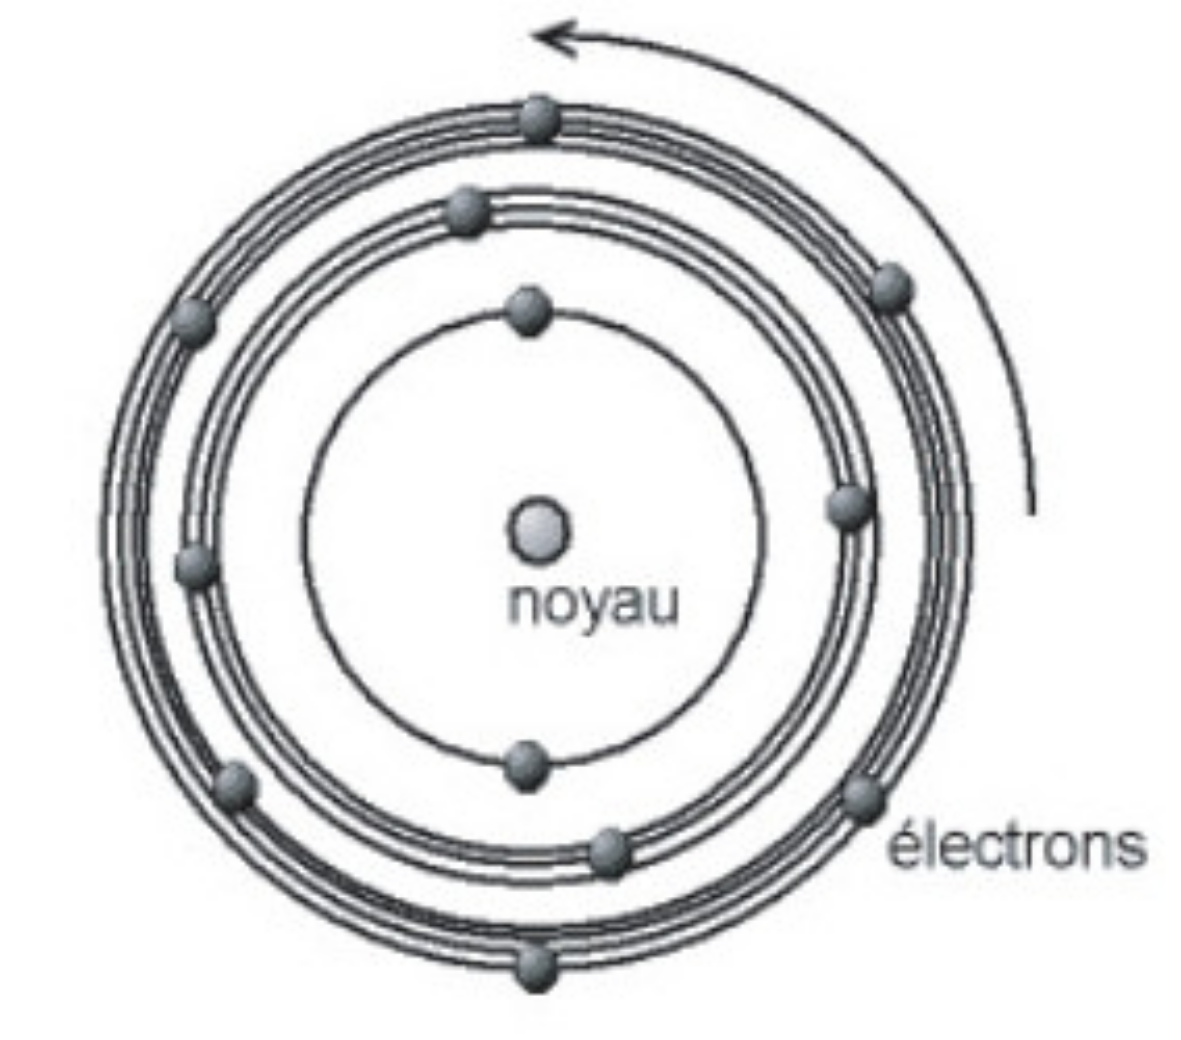
\includegraphics[width=\linewidth]{mod_bohr-plain}
		\end{center}
	\end{minipage}
	Une orbitale électronique correspond à une valeur de l'entier $n$. Elle est
	caractérisée par un rayon $r_n$, une vitesse $v_n$ et une énergie mécanique
	$\Ec_{m}(n)$.
	\smallbreak
	Ce modèle semi-classique n'est pas complètement satisfaisant, mais il prédit
	le spectre de raies de l'atome d'hydrogène.
	On rappelle qu'un atome d'hydrogène est constitué d'un noyau (charge $e =
		\SI{1.602e-19}{C}$, masse $m_p$) et d'un électron (charge $-e$, masse $m_e =
		\SI{9.11e-31}{kg}$). On donne les valeurs numériques de la célérité de la
	lumière dans le vide $c = \SI{3.00e8}{m.s^{-1}}$ et la permittivité
	diélectrique du vide $\ep_0 = \SI{8.85e-12}{F.m^{-1}}$.
}

\QR{%
	Rappeler l'expression de la force d'interaction exercée par le noyau sur
	l'électron et de l'énergie potentielle dont elle dérive.
}{%
	Avant toute chose, on étudie le mouvement de l'électron dans le référentiel
	lié au noyau, supposé galiléen. L'électron est animé d'un mouvement circulaire
	et uniforme de centre O. On l'étudie en coordonnées polaires d'origine O. Dans
	ce système de coordonnées, et avec $\rp = 0$, on a~:
	\begin{gather*}
		\OM = r\ur
		\qet
		\vf = r \tp\ut
		\qet
		\af = -\frac{v^2}{r}\ur
	\end{gather*}
	La seule force dont il faut tenir compte est la force d'interaction
	coulombienne qu'exerce le noyau de charge $+e$ sur l'électron de charge $-e$~:
	\begin{gather*}
		\Ff_c = -\frac{e^2}{4\pi\ep_0r^2}\ur
		\Ra
		\Ec_{p,c} = -\frac{e^2}{4\pi\ep_0r}
	\end{gather*}
	On peut négliger l'interaction gravitationnelle face à cette force.
}

\QR{%
Utiliser le fait que les orbitales soient circulaires pour exprimer le carré
$v_n{}^2$ de la vitesse de l'électron en fonction de la distance $r_n$.
}{%
On projette le PFD sur $\ur$~:
\begin{gather*}
	-m_e \frac{v_n{}^2}{r_n} = -\frac{e^2}{4\pi\ep_0r^2}
	\Lra
	\boxed{v_n{}^2 = \frac{e^2}{4\pi\ep_0m_er_n}}
\end{gather*}

}
\QR{%
	Utiliser la quantification du moment cinétique pour exprimer le rayon de la
	trajectoire en fonction de $n$, $h$, $m_e$ et $e$.
}{%
	On a le module du moment cinétique~:
	\begin{gather*}
		\Lc_{O_n} = m_er_nv_n = \frac{nh}{2\pi}
		\Lra
		v_n = \frac{nh}{2\pi m_er_n}
		\\\Ra
		\frac{e^2}{4\pi\ep_0m_er_n} = \frac{n^2h^2}{4\pi^2m_e{}^2r^2}
		\\\Lra
		\boxed{r_n = \frac{n^2h^2\ep_0}{\pi m_ee^2}}
	\end{gather*}
}

\QR{%
	Calculer sa valeur pour $n=1$.
}{%
	\vspace{-15pt}
	\begin{gather*}
		\beforetext{On trouve}
		\xul{r_1 = \SI{52}{pm}}
	\end{gather*}
}

\QR{%
	Exprimer l'énergie mécanique $\Ec_m(n)$ de l'électron et montrer qu'elle se
	met sous la forme $\Ec_m(n) = -\frac{A}{n^2}$. Donner l'expression et la
	valeur numérique de $A$ en électron-volts (on rappelle que $\SI{1}{eV} =
		\SI{1.6e-19}{J}$).
}{%
	\vspace{-15pt}
	\begin{DispWithArrows*}[groups]
		\Ec_m(n) &= \Ec_c + \Ec_p
		\\\Lra
		\Ec_m(n) &=
		\frac{1}{2}m_ev_n{}^2 - \frac{e^2}{4\pi\ep_0r_n} =
		-\frac{e^2}{8\pi\ep_0r_n}
		\Arrow{$\DS r_n = \frac{n^2h^2\ep_0}{\pi m_ee^2}$}
		\\\Lra
		\Aboxed{\Ec_m(n) &= -\frac{e^4m_e}{8\ep_0{}^2h^2}\frac{1}{n^2} =
			-\frac{A}{n^2}}
		\\
		\text{avec} \quad
		\Aboxed{A &= \frac{e^4m_e}{8\ep_0{}^2h^2}}
		\Lra
		\xul{A = \SI{2.17e-18}{J} = \SI{13.6}{eV}}
	\end{DispWithArrows*}
}

\QR{%
	Sachant que le passage d'un niveau d'énergie $\Ec_m(n_2)$ à un autre
	$\Ec_m(n_1)$ se traduit par l'émission d'un photon de fréquence $\nu$ telle
	que $\Delta{E} = h\nu$, en déduire que les longueurs d'onde $\lambda$ émises
	vérifient~:
	\[
		\frac{1}{\lambda} =
		R_H \left( \frac{1}{n_2{}^2} - \frac{1}{n_1{}^2} \right)
	\]
	On rappelle que $\nu = c/\lambda$. On donnera l'expression de la constante
	de \textsc{Rydberg} $R_H$ et sa valeur numérique.
}{%
	\vspace{-15pt}
	\begin{gather*}
		\Delta{\Ec} =
		A \left( \frac{1}{n_2{}^2} - \frac{1}{n_1{}^2} \right) =
		h\nu = h \frac{c}{\lambda}
		\\\Lra
		\frac{1}{\lambda} = \frac{A}{hc}\left( \frac{1}{n_2{}^2}-\frac{1}{n_1{}^2} \right)
		\\\Lra
		\boxed{\frac{1}{\lambda} = R_H\left( \frac{1}{n_2{}^2}-\frac{1}{n_1{}^2} \right)}
		\qav
		\boxed{R_H = \frac{A}{hc} = \frac{e^4m_e}{8\ep_0{}^2ch^3}}
		\Lra
		\xul{R_H = \SI{1.09e7}{m^{-1}}}
	\end{gather*}
}

\resetQ
\section{Expérience de \textsc{Rutherford}}
\enonce{%
	Entre 1909 et 1911, Ernest \textsc{Rutherford} et ses deux étudiants Hans
	\textsc{Geiger} et Ernest \textsc{Marsden} ont réalisé et interprété une
	expérience consistant à bombarder une mince feuille d'or avec des particules
	$\alpha$ (que \textsc{Rutherford} avait précédemment identifiées comme des
	noyaux d'hélium). Ils observèrent que la plupart de ces particules
	traversaient la feuille sans être affectées (donc ne rencontraient que du
	vide), mais que certaines étaient déviées, parfois très fortement~: les angles
	de déviation pouvant être reliés aux dimensions microscopiques, cela permi la
	découverte du noyau atomique et l'estimation de sa taille.
	\smallbreak
	\noindent
	\begin{minipage}[c]{.48\linewidth}
		On considère ici une particule $\alpha$ de masse $m$ et de charge $+2e$, venant
		de l'infini avec la vitesse $\vfo = v_0\ex$, et s'approchant avec le paramètre
		d'impact $b$ d'un noyau cible de numéro atomique $Z$. La particule est repérée
		par ses coordonnées polaires $(r,\th)$ dans le plan $(\Or xy)$.
		\bigbreak
		Le noyau reste pratiquement immobile dans le référentiel terrestre~: on
		travaille dans ce référentiel supposé galiléen, le repère étant centré sur la
		position O du noyau. La trajectoire suivie par la particule $\alpha$ est une
		branche d'hyperbole représentée ci-contre.
	\end{minipage}
	\hfill
	\begin{minipage}[c]{.48\linewidth}
		\begin{center}
			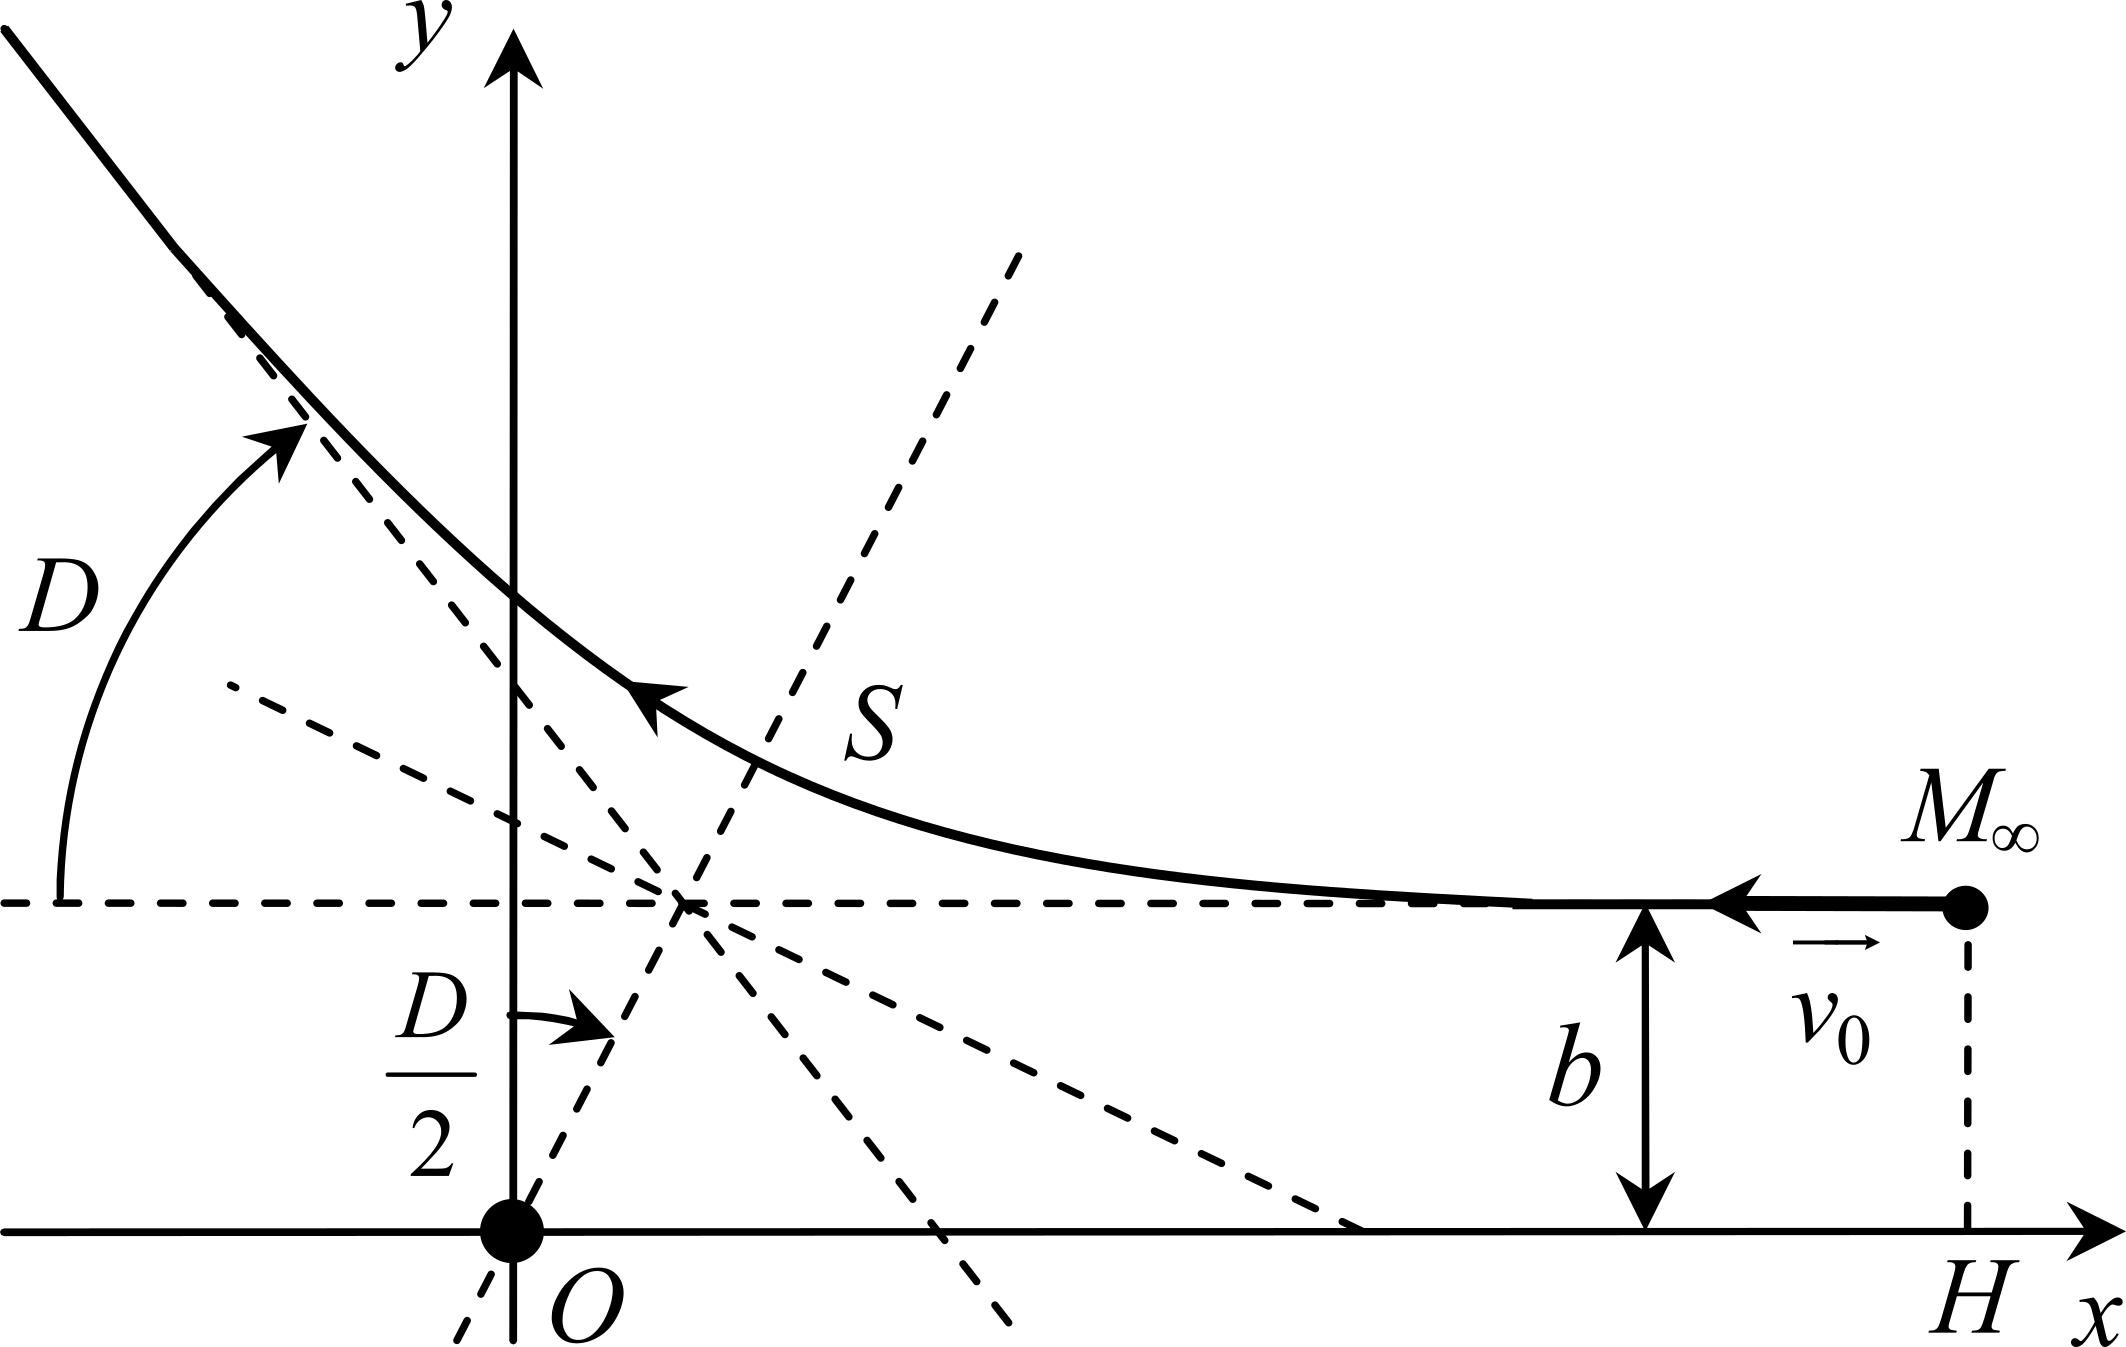
\includegraphics[width=\linewidth]{ruth-plain}
			\captionof{figure}{Trajectoire suivie par la particule $\alpha$.}
			\label{fig:ruth}
		\end{center}
	\end{minipage}
}

\QR{%
	Donner l'expression de la force électrique subie par la particule $\alpha$,
	sous la forme $\Ff = \frac{K}{r^2}\er$ ainsi que celle de son énergie
	potentielle d'interaction.
}{%
	\begin{gather*}
		\boxed{\Ff = \frac{1}{4\pi\ep_0}\frac{2Ze^2}{r^2}\er} \Ra K =
		\frac{Ze^2}{2\pi\ep_0}
		\qet
		\boxed{\Ec_p = \frac{1}{4\pi\ep_0}\frac{2Ze^2}{r}}
	\end{gather*}
}

\QR{%
	Montrer que l'énergie mécanique $\Ec_m$ de la particule $\alpha$ est une
	constante du mouvement et donner sa valeur.
}{%
	Particule soumise uniquement à $\Ff$ conservative, donc $\Ec_m = \cte$, ainsi
	\begin{gather*}
		\Ec_m = \cte
		\Lra
		\Ec_c + \Ec_p(r) = \cte
		\Lra
		\frac{1}{2}mv^2 + \frac{1}{2\pi\ep_0}\frac{Ze^2}{r} = \cte
		\\
		\beforetext{Or initialement}
		v(0) \to v_0
		\qet
		r(0) \to \infty
		\Ra
		\boxed{\Ec_m = \frac{1}{2}mv_0{}^2}
	\end{gather*}
}

\QR{%
	Montrer que le moment cinétique $\Lcf_{\Or}$ de la particule $\alpha$ en O est
	un vecteur constant, et donner la valeur de cette constante à l'aide des
	conditions initiales. Montrer que $\Lcf_{\Or}$ s'exprime de manière simple en
	fonction des variables $r$ et $\tp$.
}{%
	\vspace{-15pt}
	\begin{gather*}
		\dv{\Lcf_{\Or}}{t} =
		\OM \wedge \underbracket[1pt]{\Ff}_{\mathclap{\parr \OM}} = \of
		\Lra
		\boxed{\Lcf_{\Or} = \vcte}
		\\
		\beforetext{Or}
		\Lcf_{\Or}(0) = (x_0\ex+b\ey)\wedge (-mv_0\ex)
		\Lra
		\boxed{\Lcf_{\Or} = mbv_0\ez}
		\\
		\beforetext{De plus,}
		\Lcf_{\Or} = r\er \wedge (\rp \er+ r \tp \et)
		\Lra
		\boxed{\Lcf_{\Or} = mr^2 \tp \ez}
		\qquad \text{(et $r^2 \tp = b v_0$)}
	\end{gather*}
}

\QR{%
	Montrer que l'énergie mécanique peut se mettre sous la forme $\Ec_m =
		\frac{1}{2}m \rp^2 + \Ec_p'(r)$ et expliciter la fonction $\Ec_p'(r)$.
	Comment l'appelle-t-on~?
}{%
	\vspace{-15pt}
	\begin{gather*}
		\Ec_m = \frac{1}{2}m(\rp^2 + r^2 \tp^2) + \Ec_p(r)
		\\\Lra
		\Ec_m =
		\frac{1}{2}m \left( \rp^2 + \frac{b^2v_0{}^2}{r^2} \right) +
		\frac{1}{2\pi\ep_0}\frac{Ze^2}{r}
		\\\Lra
		\boxed{\Ec_m = \frac{1}{2}m \rp^2 + \Ec_{p,\rm eff}(r)}
		\qav
		\boxed{\Ec_{p,\rm eff}(r) =
		\frac{1}{2}m \frac{b^2v_0{}^2}{r^2}  + \frac{1}{2\pi\ep_0}\frac{Ze^2}{r}
		}
	\end{gather*}
	On l'appelle l'\textbf{énergie potentielle effective} (ou efficace).
}

\QR{%
On note S la position de la particule $\alpha$ pour laquelle elle passe au
plus près du noyau d'or, et on note $r_{\min} = \rm OS$ la distance minimale
d'approche. Que revient l'expression de $\Ec_m$ lorsque $r = r_{\min}$~? En
déduire que
\[
	r_{\min} = \frac{K}{mv_0{}^2}
	\pac{1 + \sqrt{1 + \left( \frac{mbv_0{}^2}{K} \right)^2}}
\]
}{%
Lorsque $r$ est minimal, sa dérivée est nulle donc $\Ec_m = \Ec_{p,\rm
		eff}(r_{\min})$. Ainsi,
\smallbreak
\begin{isd}[lefthand ratio=.55]
	\begin{align*}
		\Ec_m                                           & = \frac{1}{2}\frac{mb^2v_0{}^2}{r_{\min}{}^2} + \frac{1}{2\pi\ep_0}
		\frac{2e^2}{r_{\min}}
		\\\Lra
		\frac{1}{2}mv_0{}^2                             & = \frac{1}{2} \frac{mb^2v_0{}^2}{r_{\min}^2} +
		\frac{K}{r_{\min}}
		\\\Lra
		mv_0{}^2r_{\min}{}^2 - 2Kr_{\min} - mb^2v_0{}^2 & = 0
	\end{align*}
	\tcblower
	\begin{DispWithArrows*}[groups]
		\Ra
		\Delta   & = K^2 + (mbv_0{}^2) > 0
		\Arrow{$r_{\min} > 0$}
		\\\Ra
		r_{\min} & = \frac{K + \sqrt{K^2 + (mbv_0{}^2)^2}}{mv_0{}^2}
		\\\Lra
		\Aboxed{
		r_{\min} & = \frac{K}{mv_0{}^2}
		\pac{1 + \sqrt{1 + \left( \frac{mbv_0{}^2}{K} \right)^2}}
		}
	\end{DispWithArrows*}
\end{isd}
}

\QR{%
On donne $\ep_0 = \SI{8.9e-12}{F.m^{-1}}$, $e = \SI{1.6e-19}{C}$, $m =
	\SI{6.6e-27}{kg}$, $v_0 = \SI{2.0e7}{m.s^{-1}}$ et $Z = 79$ pour l'or. D'autre
part, on peut montrer que l'angle de déviation $D$ de la particule est donné
par la relation
\[
	\tan(\frac{D}{2}) = \frac{K}{mbv_0{}^2}
\]
Calculer $b$ puis $r_{\min}$ pour $D_1 = \ang{60}$ et pour $D_2 = \ang{180}$
(particule envoyée vers l'arrière). En déduire l'ordre de grandeur de la
taille du noyau d'or.
}{%
\begin{gather*}
	\boxed{b = \frac{K}{mv_0{}^2\tan(D/2)} =
	\frac{2e^2}{2\pi\ep_0mv_0{}^2 \tan(D/2)}}
	\\\AN
	\xul{b_1 = \SI{2.4e-14}{m}}
	\qet
	\xul{b_2 = 0}
	\qqdc
	\xul{r_{\min,1} = \SI{2.4e-14}{m}}
	\qet
	\xul{r_{\min,2} = \SI{2.7e-14}{m}}
\end{gather*}
La taille caractéristique du noyau d'or (assez gros) est donc de l'ordre de
\fbox{\SI{e-14}{m}}, soit environ \num{10000} fois plus petit que l'atome.
}

\end{document}
